\documentclass{beamer}

\makeatletter
\renewcommand<>\beamer@framefootnotetext[1]{%
  \global\setbox\beamer@footins\vbox{%
    \hsize\framewidth
    \textwidth\hsize
    \columnwidth\hsize
    \unvbox\beamer@footins
    \reset@font\footnotesize
    \@parboxrestore
    \protected@edef\@currentlabel
         {\csname p@footnote\endcsname\@thefnmark}%
    \color@begingroup
      \uncover#2{\@makefntext{%
        \rule\z@\footnotesep\ignorespaces\parbox[t]{.9\textwidth}{#1\@finalstrut\strutbox}\vskip1sp}}%
    \color@endgroup}%
}
\makeatother

\usetheme{Berkeley}
\usepackage{media9}
\usepackage{hyperref}
\usepackage{movie15}
\setbeamertemplate{caption}[numbered]
\setbeamertemplate{bibliography item}{\insertbiblabel}
\usepackage{siunitx}
\usepackage{multirow}
 \usepackage{graphicx}

\numberwithin{equation}{section}
\numberwithin{figure}{section}


\title{Simulation of flow over a bridge using OpenFOAM}
\author{Sahl Abdelsayed}
\institute{University of Sheffield}
\date{\today}

\begin{document}


\begin{frame}
\titlepage
\end{frame}

\begin{frame}
\frametitle{Outline}
\tableofcontents
\end{frame}

\section{Introduction}

\begin{frame}

\frametitle{Introduction}

\begin{block}{What is OpenFOAM?}
OpenFOAM (Open source Field Operation And Manipulation) is a free, open-source, customisable CFD numerical solver.
\end{block}

\pause
We need some context...

\end{frame}



\section{Engineering aim}

\begin{frame}
\frametitle{A bit of context}
In 1879, Tay bridge in Dundee Scotland has collapsed due to a violent storm \cite{biezma2007collapse}.
\begin{figure}
\centering 
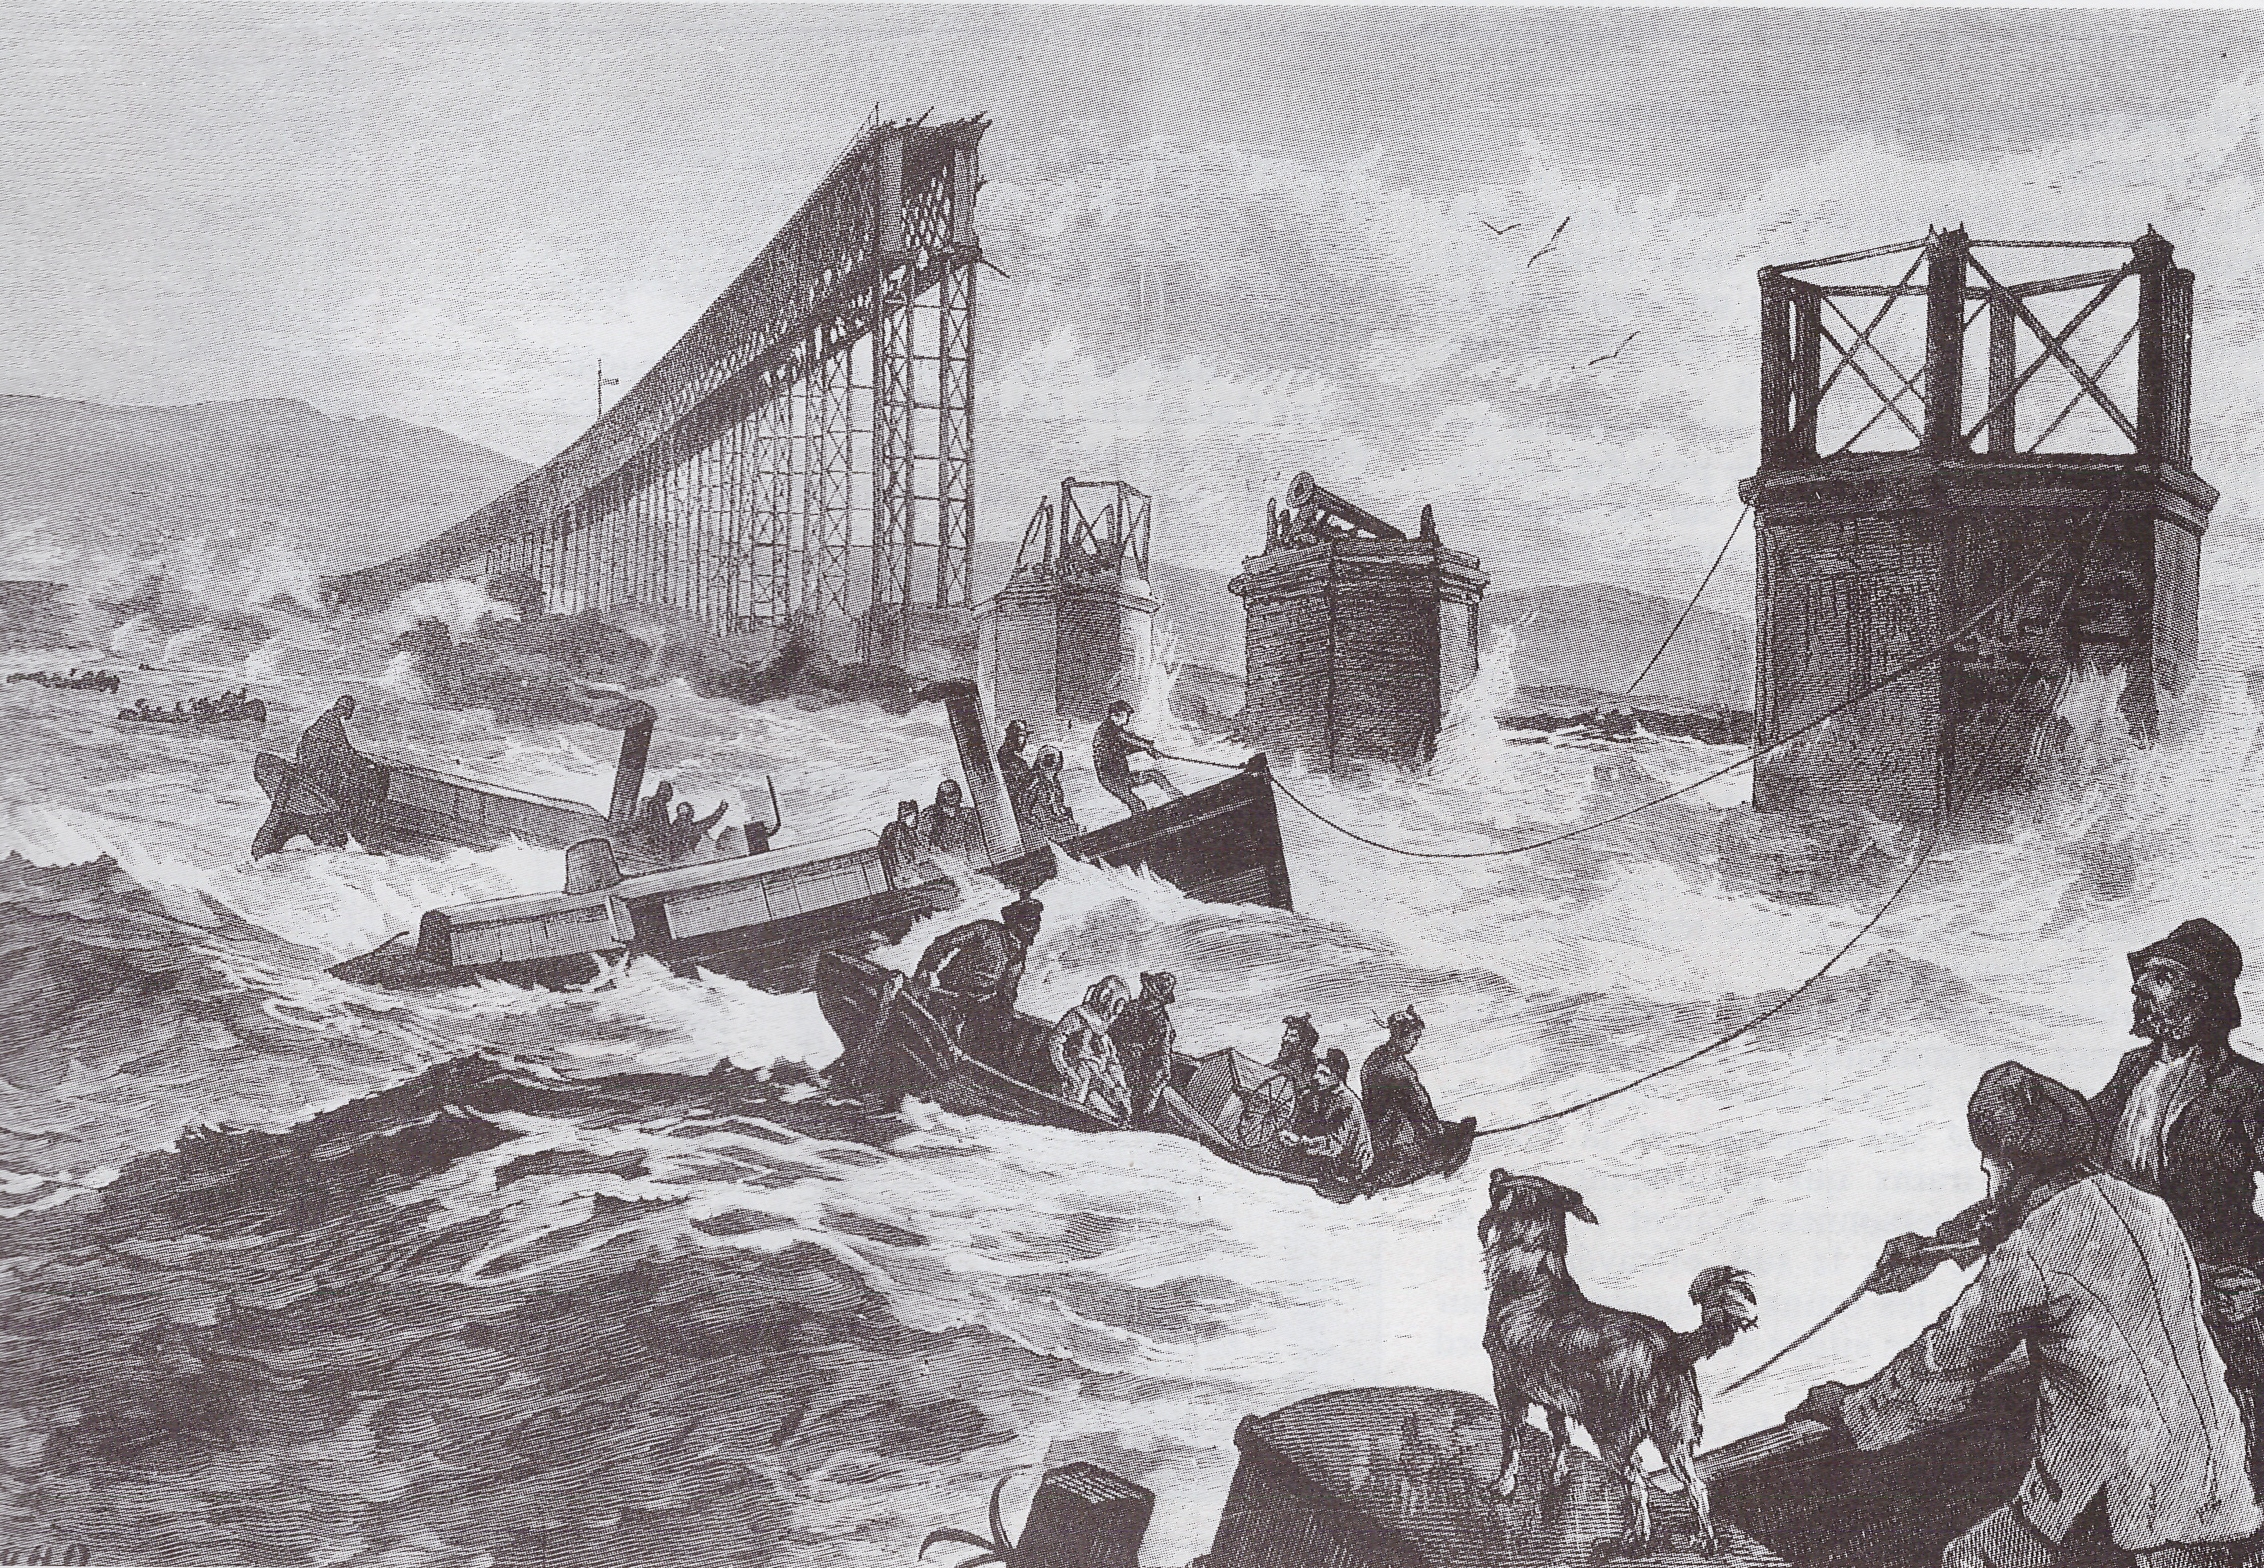
\includegraphics[width=0.75\textwidth]{bridge.jpeg}
\end{figure}
\end{frame}

\begin{frame}
\frametitle{A bit of context}
\href{https://www.youtube.com/watch?v=XggxeuFDaDU}{Tacoma Narrows Bridge} has collapsed in an unexpected manner in 1940.
\begin{figure}
    \centering
    \includemedia[
    width=1.0\linewidth,height=0.5\linewidth,
    activate=pageopen,
    flashvars={
        modestbranding=1 % no YT logo in control bar
        &autohide=1 % controlbar autohide
        &showinfo=0 % no title and other info before start
        &rel=0 % no related videos after end
    }
        ]{}{http://www.youtube.com/v/XggxeuFDaDU}
\end{figure}
\end{frame}

\begin{frame}
\frametitle{More about the Tacoma Bridge}
The initial theory of failure was that the bridge collapsed due to resonance.\\~\\
\pause 
This theory turned out to be incorrect and the failure was due to aeroelastic flutter \cite{green2006failure}.\\~\\
\pause
\begin{block}{Engineering aim of this project is..}
Improving the fundamental understanding of flow past a bridge by carrying out the appropriate simulations.
\end{block}
\pause
As we all know, simulations bring about numerous advantages.
\end{frame}


\section{Setting up the Simulation}
\begin{frame}
\frametitle{Aims and assumptions} 
\textbf{\Large Project aims}
\begin{itemize}
\item Simplify the geometry to a simple 2D cylinder model.
\pause
\item Run and analyse simulations on Re=20, Re=50, Re=100. \\~\\
\pause 
\end{itemize}
\pause
\textbf{\Large Assumptions}
\pause
\begin{itemize}
\item Flow is laminar.
\pause
\item Flow is incompressible.
\pause
\item Air is a Newtonian fluid. 
\pause
\item Flow is transient, single phase, and isothermal. 
\end{itemize}
\end{frame}

\begin{frame}
\frametitle{Geometry}
The geometry was drawn on an application called \textbf{gmsh}. \\~\\
\pause
The cylinder has a diameter of 1\si{\meter}. \\~\\
\pause
The outline of the 2D cylinder  is drawn shown in Figure~\ref{Geo1}.
\pause
\begin{figure}
\centering 
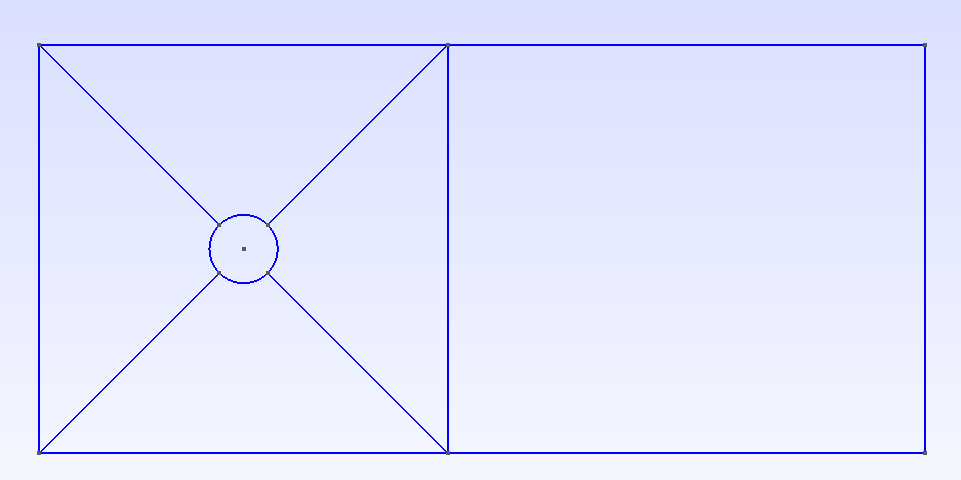
\includegraphics[width=0.75\textwidth]{Geometry1.png}
\caption{Shows the outline of the cylinder}
\label{Geo1}
\end{figure}
\end{frame}

\begin{frame}
\frametitle{Geometry}
The next stage involved extruding the geometry. \\~\\
\pause
Extrusion is important as it will add surfaces as shown in Figure~\ref{Geo2}.
\begin{figure}
\centering 
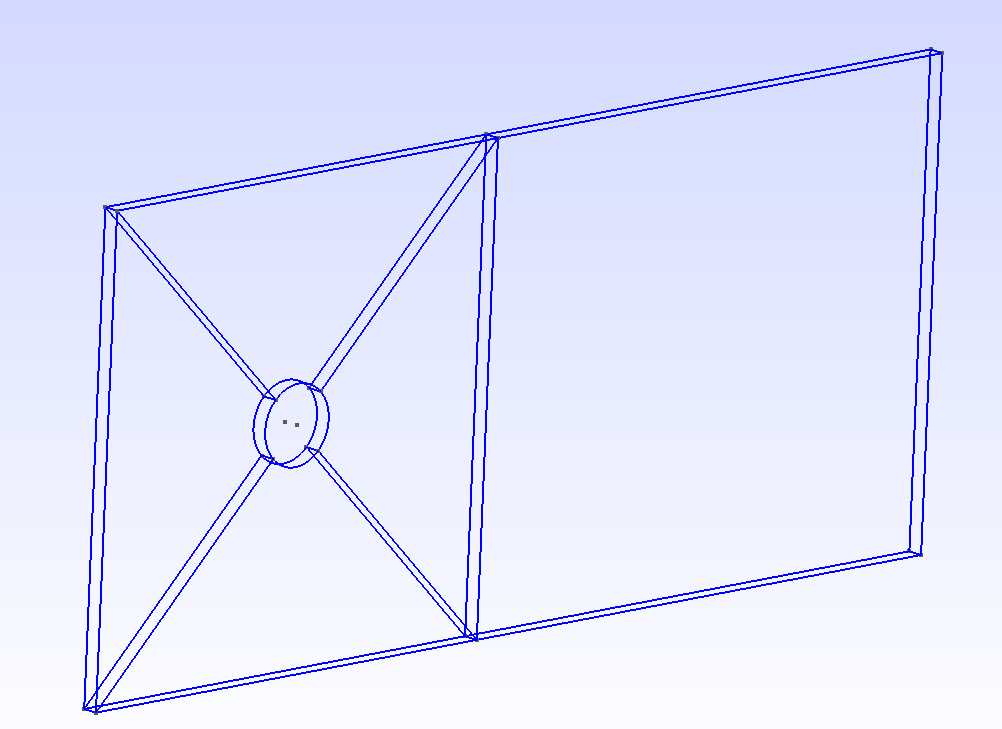
\includegraphics[width=0.6\textwidth]{Geometry2.png}
\caption{Shows the extruded cylinder.}
\label{Geo2}
\end{figure}
\end{frame}

\begin{frame}
\frametitle{Geometry}
After the extrusion the geometry was meshed. \\~\\
\pause
The result obtained are shown in Figure~\ref{Geo3}.
\begin{figure}
\centering 
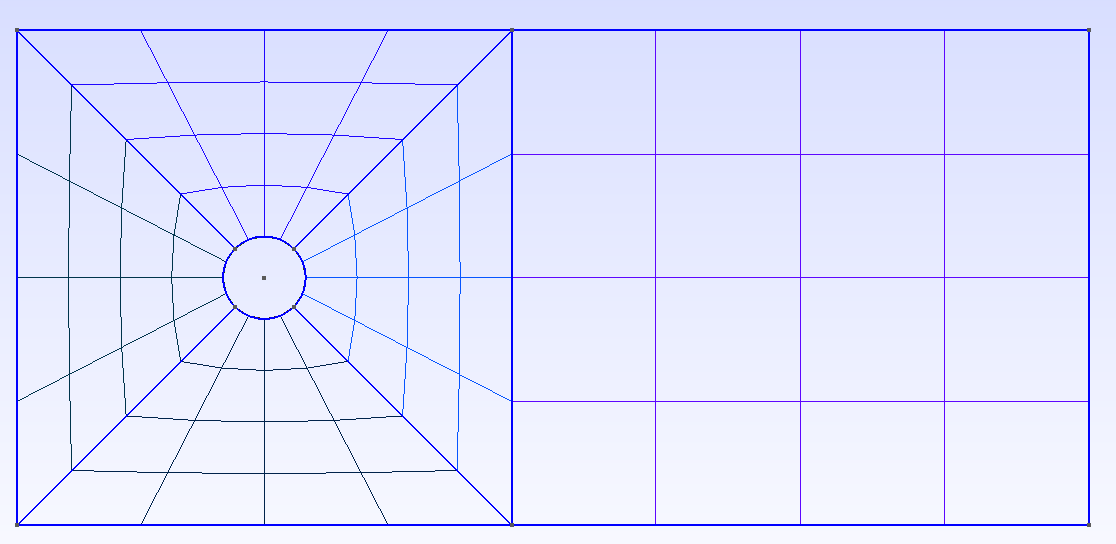
\includegraphics[width=0.75\textwidth]{Geometry3.png}
\caption{Shows the cylinder with the applied meshing.}
\label{Geo3}
\end{figure}
\end{frame}

\begin{frame}
\frametitle{Geometry}
Afterwards, the surfaces were labelled as shown on Figure~\ref{Geo4} \\~\\
\pause
This is an important step as it plays a big role in setting the boundary conditions.
\begin{figure}
\centering 
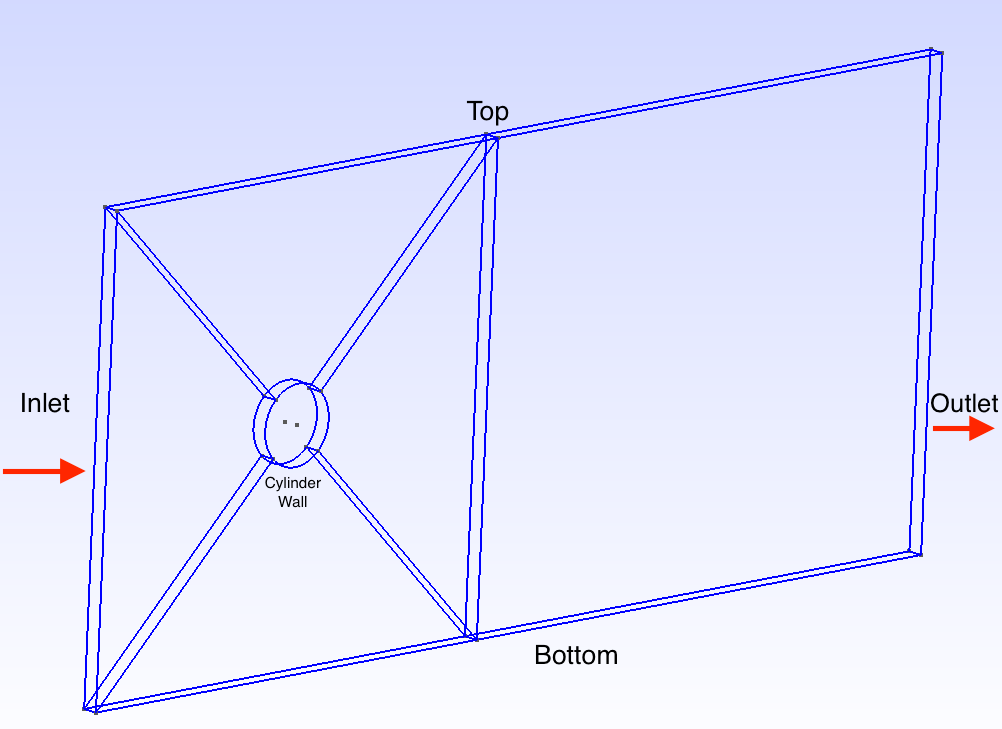
\includegraphics[width=0.6\textwidth]{Geometry4.png}
\caption{Shows the final geometry with labelled surfaces}
\label{Geo4}
\end{figure}
\end{frame}

\begin{frame}
\frametitle{Boundary conditions}
\pause 
\textbf{Velocity boundary conditions:}
\begin{itemize}
\pause
\item 1 \si{\meter\per\second} in the x-direction at the inlet, to be able to apply non-dimensionalisation.
\pause 
\item 0 \si{\meter\per\second} at cylinder wall.
\pause
\item Slip condition on top and bottom.
\pause
\item Zero gradient at the outlet. 
\pause
\item Back and front wall were set as empty.
\end{itemize}
\end{frame}

\begin{frame}
\frametitle{Boundary conditions}
\textbf{Pressure boundary conditions:}
\pause
\begin{itemize}
\item The following surfaces were set as zero gradient:
\pause
\begin{itemize}
\item Top and bottom
\item Inlet
\item Cylinder wall
\end{itemize}
\pause
\item Back and front walls were set as empty
\pause
\item Outlet was set to 0 \\~\\
\end{itemize} 
\pause
To understand why outlet was set to 0, the Navier-Stokes equation should be studied.
\end{frame}

\begin{frame}
\frametitle{Navier-Stokes equations}
\pause
The mass continuity equation can be written as \footnote{$\rho$ is the density and $\overrightarrow{\textbf V}$ is the velocity vector.\\}
\pause
\begin{equation}
\frac{\partial \rho}{\partial t} + {\nabla}\cdot(\rho \overrightarrow{\textbf V})=0  
\label{eq:1}
\end{equation}

Since the flow is incompressible Equation~\ref{eq:1} can be written as
\pause
\begin{equation}
  {\nabla}\cdot(\overrightarrow{\textbf V}) =0 
\label{eq:2}
\end{equation}

\end{frame}

\begin{frame}
\frametitle{Navier-Stokes equations} 
Navier-stokes momentum equation can be expressed as \footnote{$\rho$ is the density, $\overrightarrow{\textbf V}$ is the velocity vector, $\overline{P}$ is the pressure, and $\mu$ is the dynamic viscosity.}
\begin{equation}
\frac{\partial (\rho \overrightarrow{\textbf V})}{\partial t} + \rho {\nabla}\cdot(\overrightarrow{\textbf V} \overrightarrow{\textbf V})= - {\nabla} \overline{P} + \mu({\nabla^2{\overrightarrow {\textbf V}})}
\label{eq:3}
\end{equation}

Dividing by $\rho$ on both sides Equation~\ref{eq:3} can be written as \footnote{$\overline{p}$ is the pressure per unit density and $\nu$ is the kinematic viscosity.\\}

\begin{equation}
\frac{\partial ( \overrightarrow{\textbf V})}{\partial t} +  {\nabla}\cdot(\overrightarrow{\textbf V} \overrightarrow{\textbf V})= - {\nabla} \overline{p} + \nu({\nabla^2{\overrightarrow {\textbf V}})}
\label{eq:4}
\end{equation}

\end{frame}

\begin{frame}
\frametitle{Non-dimensionalisation}
\begin{block}{Definition}
Non-dimensionalisation is the process of eliminating units by suitable substitution.
\end{block}
Non-dimensionalisation facilitated setting the Reynolds number of each flow.
\end{frame}

\begin{frame}
\frametitle{Non-dimensionalisation}
For instance, Reynolds can be calculated by the following expression. \footnote{D is the diameter of the cylinder\\ and u is the velocity in the x-direction}
\pause
\begin{equation}
Re=\frac{ u D}{\nu}
\label{eq:5}
\end{equation}

\pause
Rearranging the equation to make $\nu$ subject of the formula Equation~\ref{eq:5} becomes
\pause
\begin{equation}
\nu=\frac{u D}{Re}
\label{eq:6}
\end{equation}\\~\\
\pause
It is already established that u= 1\si{\meter\per\second} and D= 1\si{\meter}\\~\\
\pause
Hence...
\pause
\begin{equation}
\nu=\frac{1}{Re}
\label{eq:7}
\end{equation}
\end{frame}

\begin{frame}
\frametitle{Non-dimensionalisation}
\pause
The required viscosity can now be calculated using Equation~\ref{eq:7}. \\~\\
\pause
Therefore, to obtain Reynolds number of 20, 50, and 100. \\~\\
\pause 
Kinematic viscosity should be set at 0.05, 0.02, and 0.01 respectively. \\~\\
\end{frame}


\section{Methodology}

\begin{frame}
\frametitle{Nature of the forces acting}
\pause
Two of the fundamental forces acting in any aerodynamic problems are:
\begin{itemize}
\pause
\item Lift F\textsubscript{L}, which acts in the y-direction 
\item Drag F\textsubscript{D}, which acts in the x-direction \\~\\
\end{itemize} 
\pause
Having obtained the forces, the coefficient of lift C\textsubscript{L} and coefficient of drag C\textsubscript{D} can be calculated. \footnote{A is the surface area}
\pause
\begin{equation}
C\textsubscript{L}=\frac{2 F\textsubscript{L}}{\rho u^2 A} 
\label{eq:8}
\end{equation} 
\begin{equation}
C\textsubscript{D}=\frac{2 F\textsubscript{D}}{\rho u^2 A}
\label{eq:9}
\end{equation}
\end{frame}

\begin{frame}
\frametitle{Time traces}
To be able to study the variation of coefficient of lift and drag along time, non-dimensional time \^{t} was required. It can be calculated using Equation~\ref{eq:10}
\pause
\begin{equation}
\hat{t}= \frac{tu}{D} 
\label{eq:10}
\end{equation}
\pause
We know that velocity u=1\si{\meter\per\second} and diameter D= 1\si{\meter} hence.. 

\begin{equation}
\hat{t}= t 
\label{eq:14}
\end{equation}
Time traces were then obtained by plotting coefficient of lift and coefficient of drag vs non-dimensional time.
\end{frame}


\begin{frame}
\frametitle{Vortex shedding frequency and Strouhal number}
\pause
By applying Fourier transform to the coefficient of lift time trace obtained, the vortex shedding frequency f can be obtained. \\~\\
\pause 
Having obtained the vortex shedding frequency, Strouhal number can be calculated using Equation~\ref{eq:11}
\begin{equation}
St= \frac{fD}{u}
\label{eq:11}
\end{equation}
Being given that u= 1\si{\meter\per\second} and D= 1\si{\meter} Equation~\ref{eq:11} simplifies to

\begin{equation}
St= f
\label{eq:12}
\end{equation}

The entire methodology process was done on MATLAB.
\end{frame}


%%%%%%%%%%%%%%%%%%%%%%%%%%%%%%%%%%%%%%%


\section{Results obtained}
%%%%%%%
%  Re=20   %
%%%%%%%
\begin{frame}
\frametitle{Velocity profile at Re=20}
Stable flow and short separation length.
\pause
\begin{figure}
\fbox{\includemovie{10cm}{6cm}{URe20.mp4}}
\end{figure}
\end{frame}

\begin{frame}
\frametitle{Pressure profile at Re=20}
\pause
Constant difference in pressure, which creates constant force. 
\pause
\begin{figure}
\fbox{\includemovie{10cm}{6cm}{PRe20.mp4}}
\end{figure}
\end{frame}

\begin{frame}
\frametitle{Time traces obtained at Re=20.}
Having obtained the forces, time traces were plotted as shown below 
\begin{figure}[H]
\centering
\begin{minipage}{.5\textwidth}
  \centering
  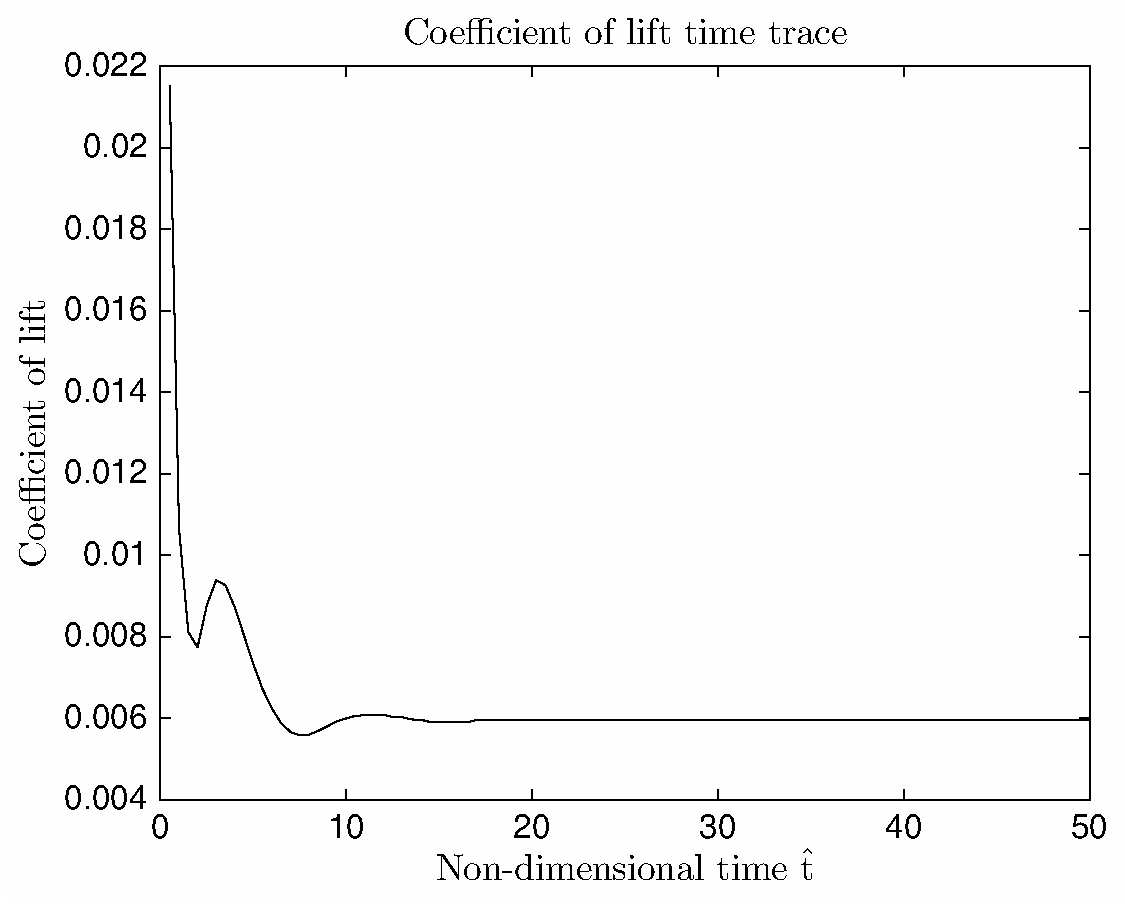
\includegraphics[scale=0.25]{Cl_20.eps}
%  \captionof{figure}{Coefficient of lift time trace.}
  %\label{fig:SRe100.1}
\end{minipage}%
\begin{minipage}{.5\textwidth}
  \centering
  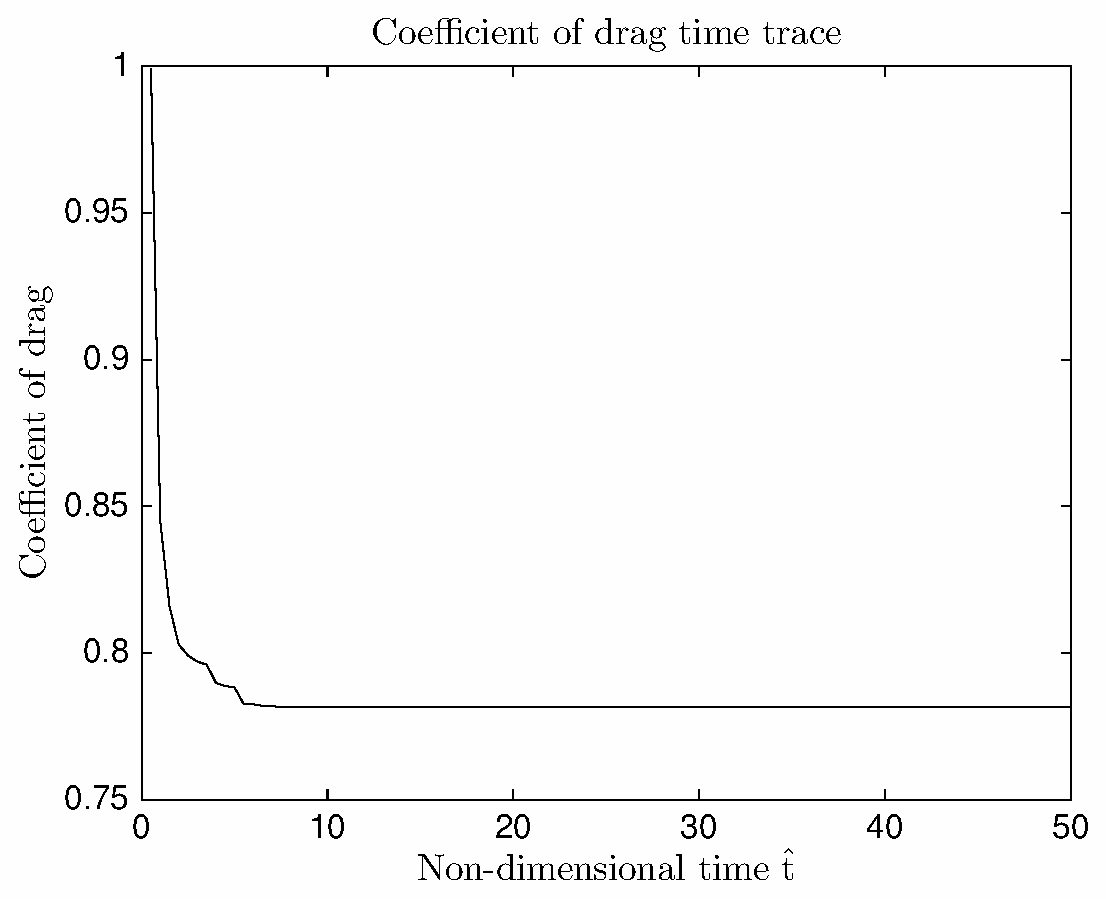
\includegraphics[scale=0.25]{Cd_20.eps}
%  \captionof{figure}{Coefficient of drag time trace.}
  %\label{fig:SRe100.2}
\end{minipage}
\end{figure}
C\textsubscript{L} = 0.006\\
C\textsubscript{D} = 0.7815
\end{frame}


\begin{frame}
\frametitle{Vortex shedding and Strouhal Number at Re=20}
Applying Fourier transformation to coefficient of lift time trace we get.. 
\begin{figure}[H]
\centering
\begin{minipage}{.5\textwidth}
  \centering
  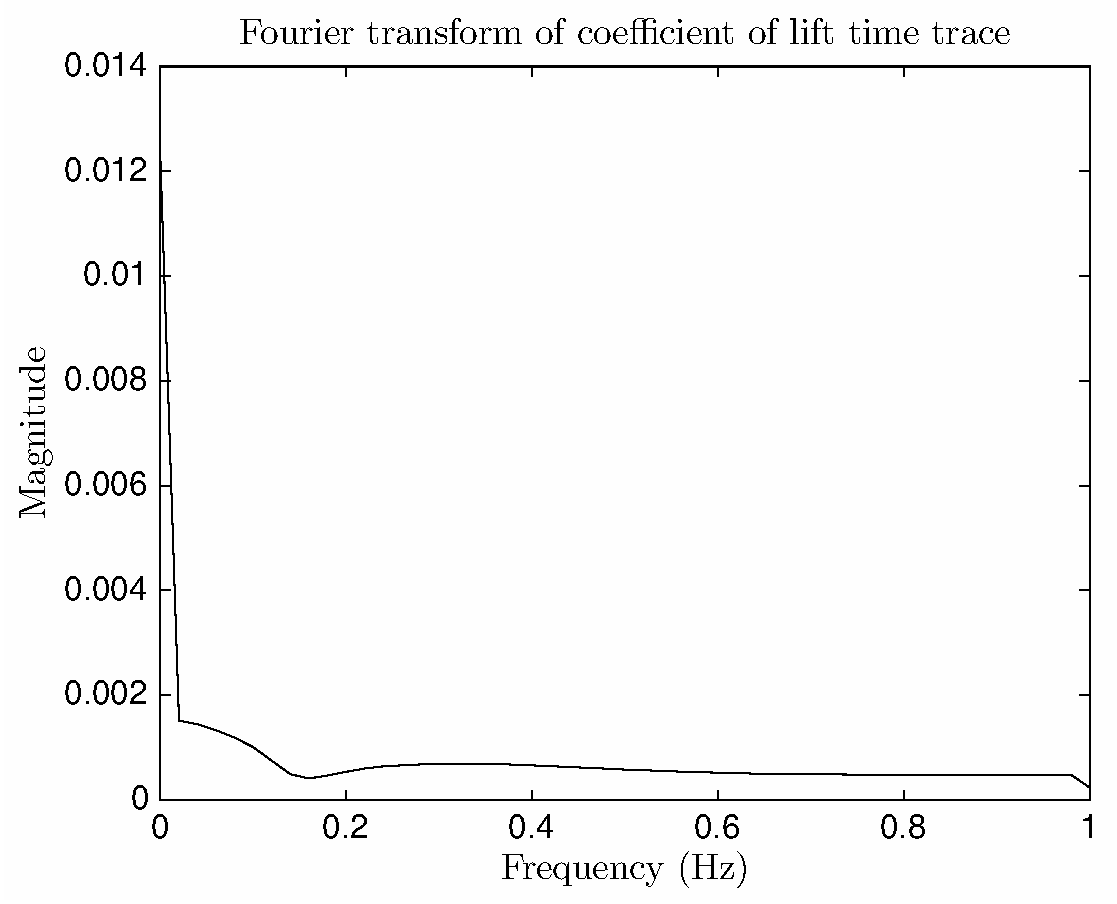
\includegraphics[scale=0.25]{FFT_20.eps}
%  \captionof{figure}{Coefficient of lift time trace.}
  %\label{fig:SRe100.1}
\end{minipage}%
\begin{minipage}{.5\textwidth}
  \centering
  \fbox{\includemovie{5cm}{5cm}{SRe20-2.mp4}}
%  \captionof{figure}{Coefficient of drag time trace.}
  %\label{fig:SRe100.2}
\end{minipage}
\end{figure}
No peaks observed, hence no vortex shedding 
\end{frame}

%%%%%%%
%  Re=50   %
%%%%%%%
\begin{frame}
\frametitle{Velocity profile at Re=50}
\pause
Initial oscillation occurs and larger separation length.
\pause
\begin{figure}
\fbox{\includemovie{10cm}{6cm}{URe50.mp4}}
\end{figure}
\end{frame}

\begin{frame}
\frametitle{Pressure profile at Re=50}
\pause
Slight fluctuation in pressure creates a slightly varying force. 
\pause
\begin{figure}
\fbox{\includemovie{10cm}{6cm}{PRe50.mp4}}
\end{figure}
\end{frame}


\begin{frame}
\frametitle{Time traces obtained at Re=50}
The time traces now can be plotted.
\begin{figure}[H]
\centering
\begin{minipage}{.5\textwidth}
  \centering
  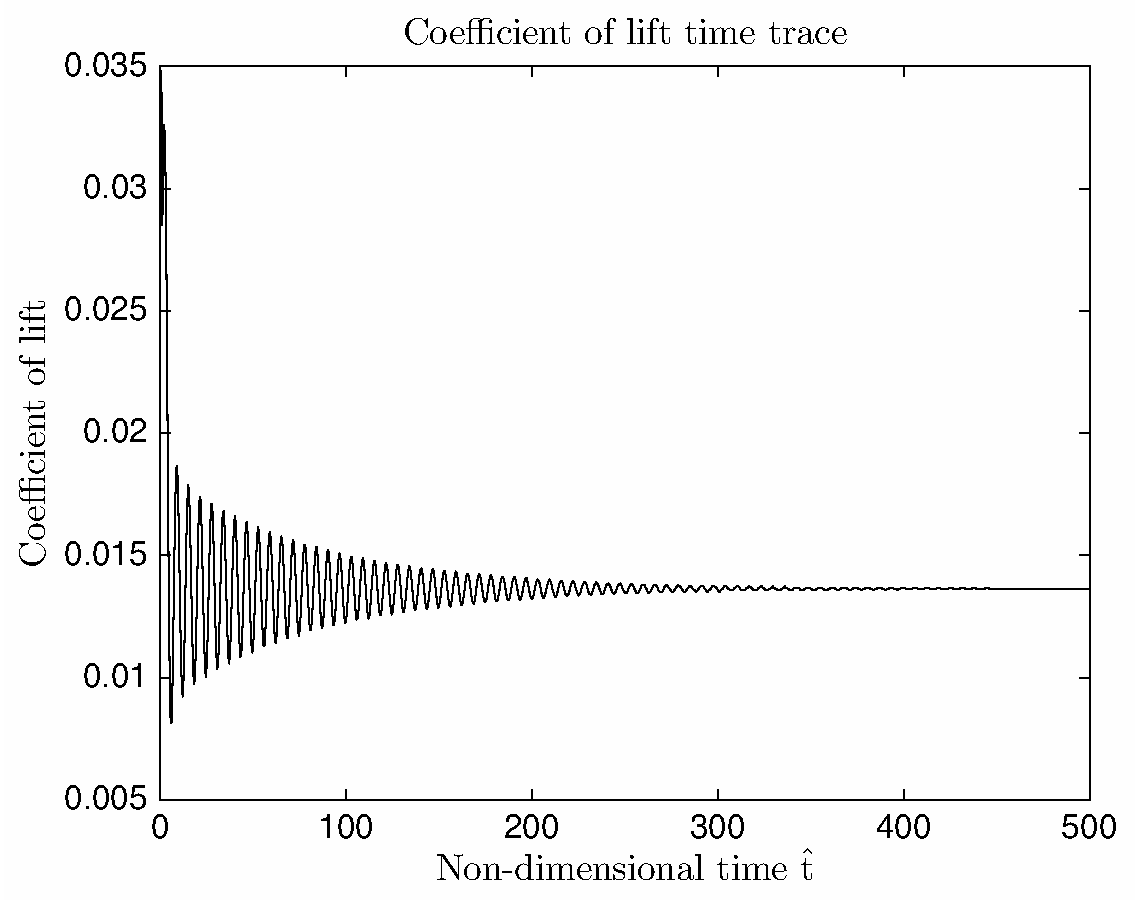
\includegraphics[scale=0.25]{Cl_50.eps}
%  \captionof{figure}{Coefficient of lift time trace.}
  %\label{fig:SRe100.1}
\end{minipage}%
\begin{minipage}{.5\textwidth}
  \centering
  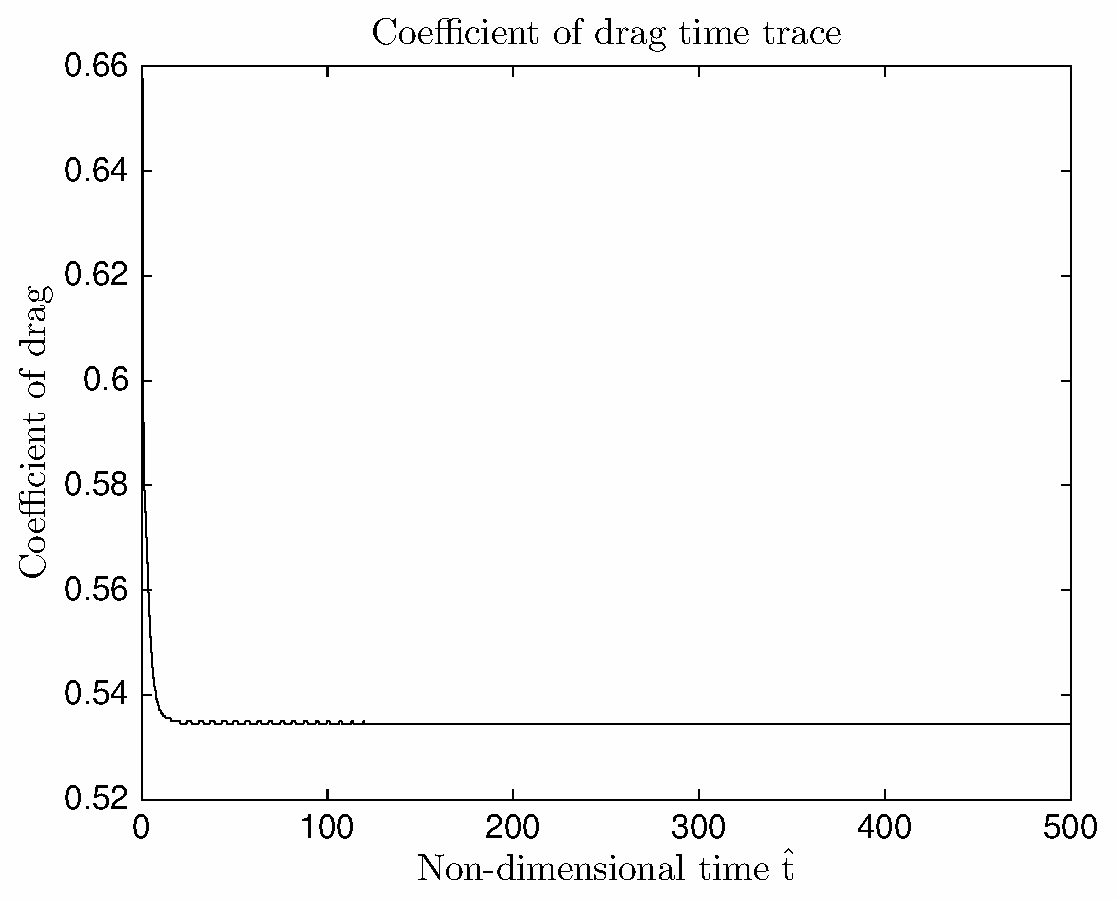
\includegraphics[scale=0.25]{Cd_50.eps}
%  \captionof{figure}{Coefficient of drag time trace.}
  %\label{fig:SRe100.2}
\end{minipage}
\end{figure}
C\textsubscript{L} = 0.0136\\
C\textsubscript{D} = 0.5345
\end{frame}

\begin{frame}
\frametitle{Vortex shedding and Strouhal Number Re=50}
Applying Fourier transformation to coefficient of lift time trace we get.. 
\begin{figure}[H]
\centering
\begin{minipage}{.5\textwidth}
  \centering
  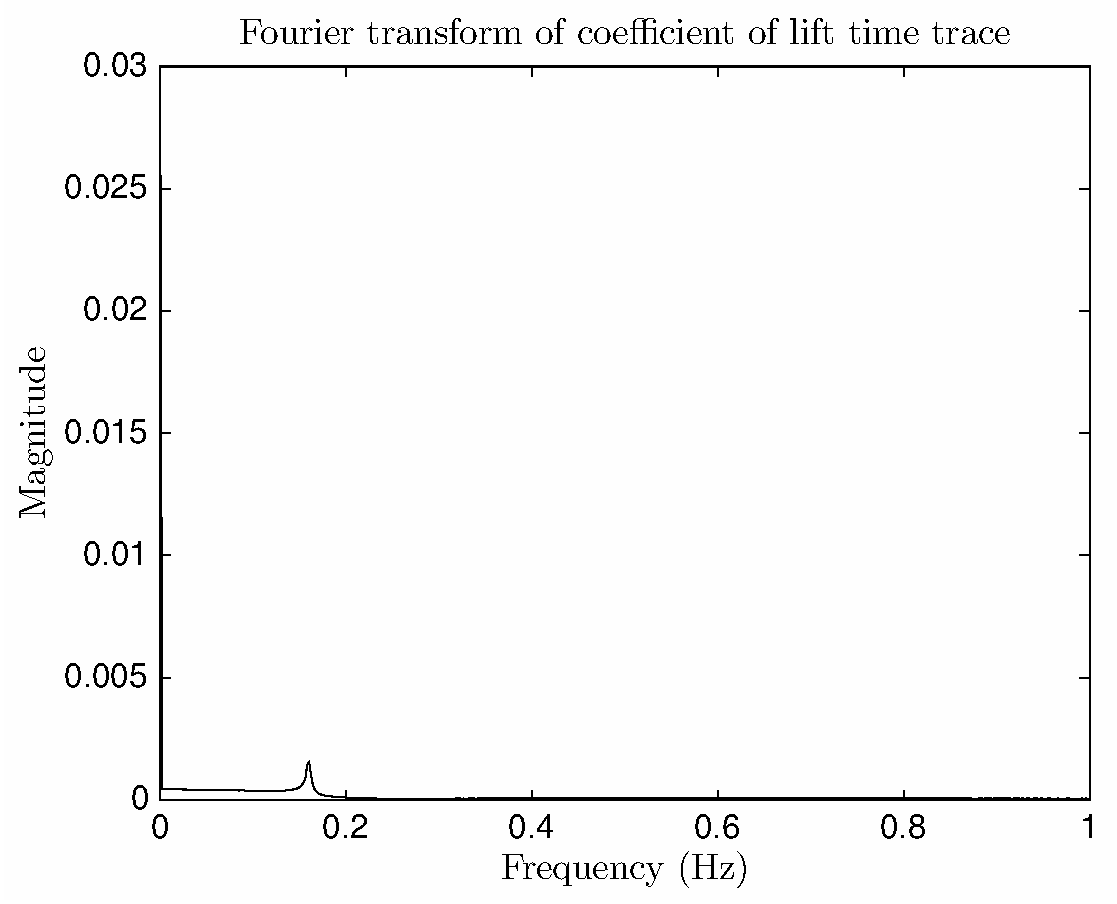
\includegraphics[scale=0.25]{FFT_50.eps}\\
%  \captionof{figure}{Coefficient of lift time trace.}
  %\label{fig:SRe100.1}
  St = f = 0.16
\end{minipage}%
\begin{minipage}{.5\textwidth}
  \centering
  \fbox{\includemovie{5cm}{6cm}{SRe50.mp4}}
%  \captionof{figure}{Coefficient of drag time trace.}
  %\label{fig:SRe100.2}
\end{minipage}
\end{figure}
\end{frame}

%%%%%%%
% Re=100   %
%%%%%%%
\begin{frame}
\frametitle{Velocity profile at Re=100}
\pause
Airflow constantly oscillating.
\pause
\begin{figure}
\fbox{\includemovie{10cm}{6cm}{URe100.mp4}}
\end{figure}
\end{frame}

\begin{frame}
\frametitle{Pressure profile at Re=100}
\pause
Fluctuation in pressure creates a fluctuating force.
\pause
\begin{figure}
\fbox{\includemovie{10cm}{6cm}{PRe100.mp4}}
\end{figure}
\end{frame}


\begin{frame}
\frametitle{Time traces obtained at Re=100}
Time traces obtained are shown below.
\begin{figure}[H]
\centering
\begin{minipage}{.5\textwidth}
  \centering
  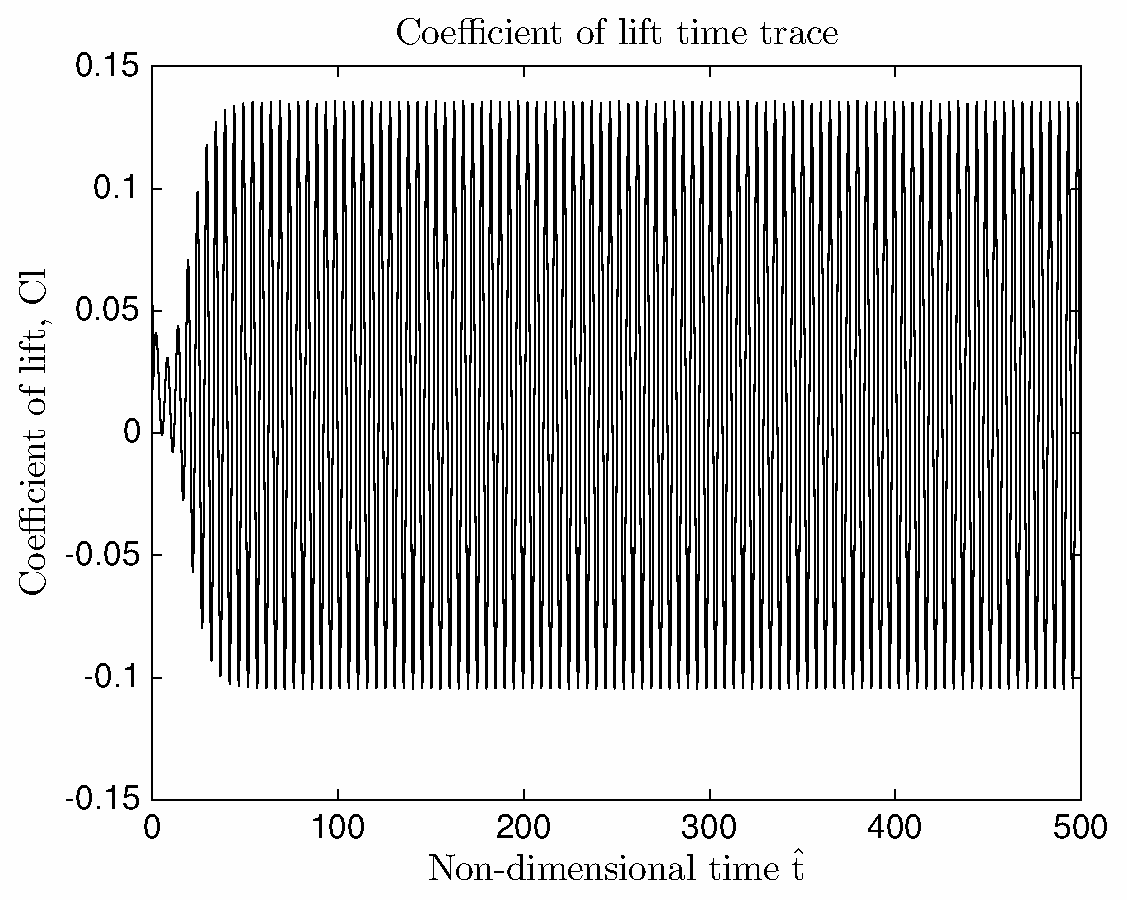
\includegraphics[scale=0.25]{Cl_100.eps}
%  \captionof{figure}{Coefficient of lift time trace.}
  %\label{fig:SRe100.1}
\end{minipage}%
\begin{minipage}{.5\textwidth}
  \centering
  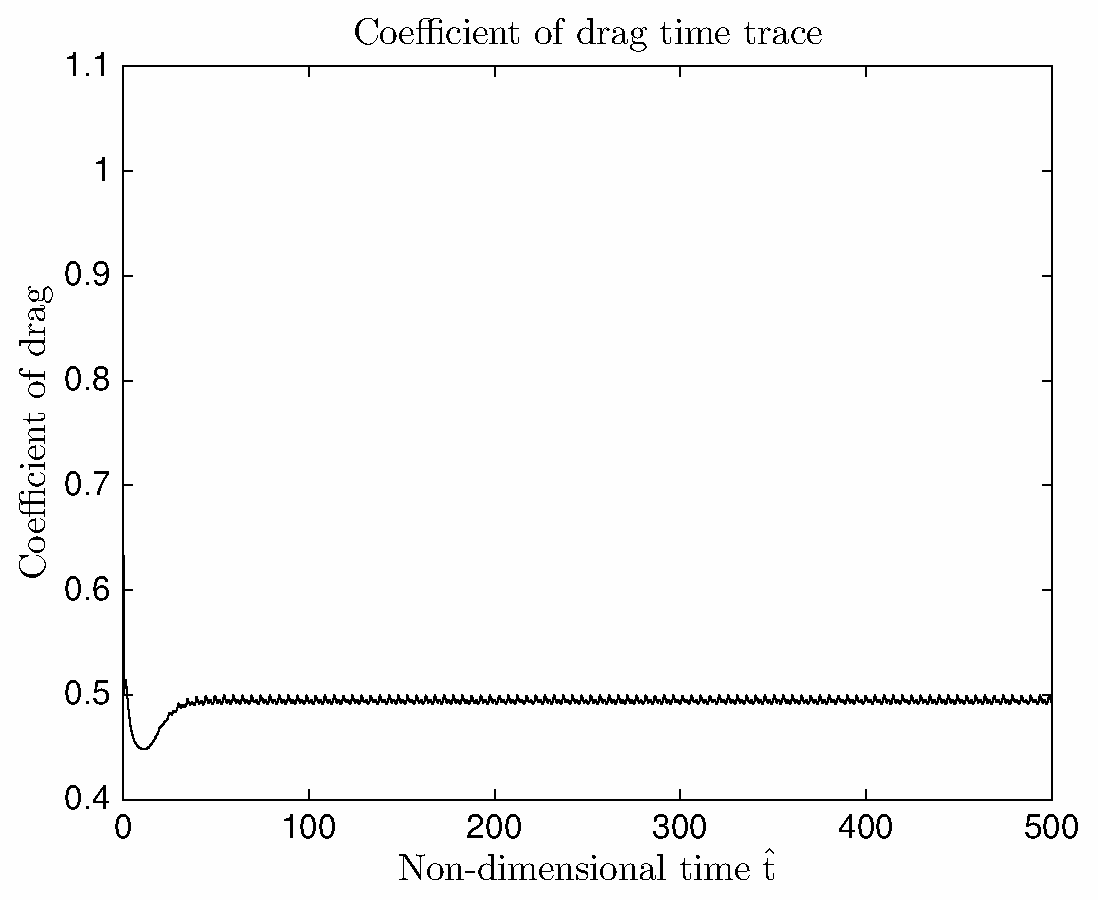
\includegraphics[scale=0.25]{Cd_100.eps}
%  \captionof{figure}{Coefficient of drag time trace.}
  %\label{fig:SRe100.2}
\end{minipage}
\end{figure}
C\textsubscript{L} = 0.136 $\leq  C\textsubscript{l} \leq$ -0.1048\\
C\textsubscript{D} = 0.493
\end{frame}

\begin{frame}
\frametitle{Vortex shedding and Strouhal number at Re=100}
Applying Fourier transformation to coefficient of lift time trace we get.. 
\begin{figure}[H]
\centering
\begin{minipage}{.5\textwidth}
  \centering
  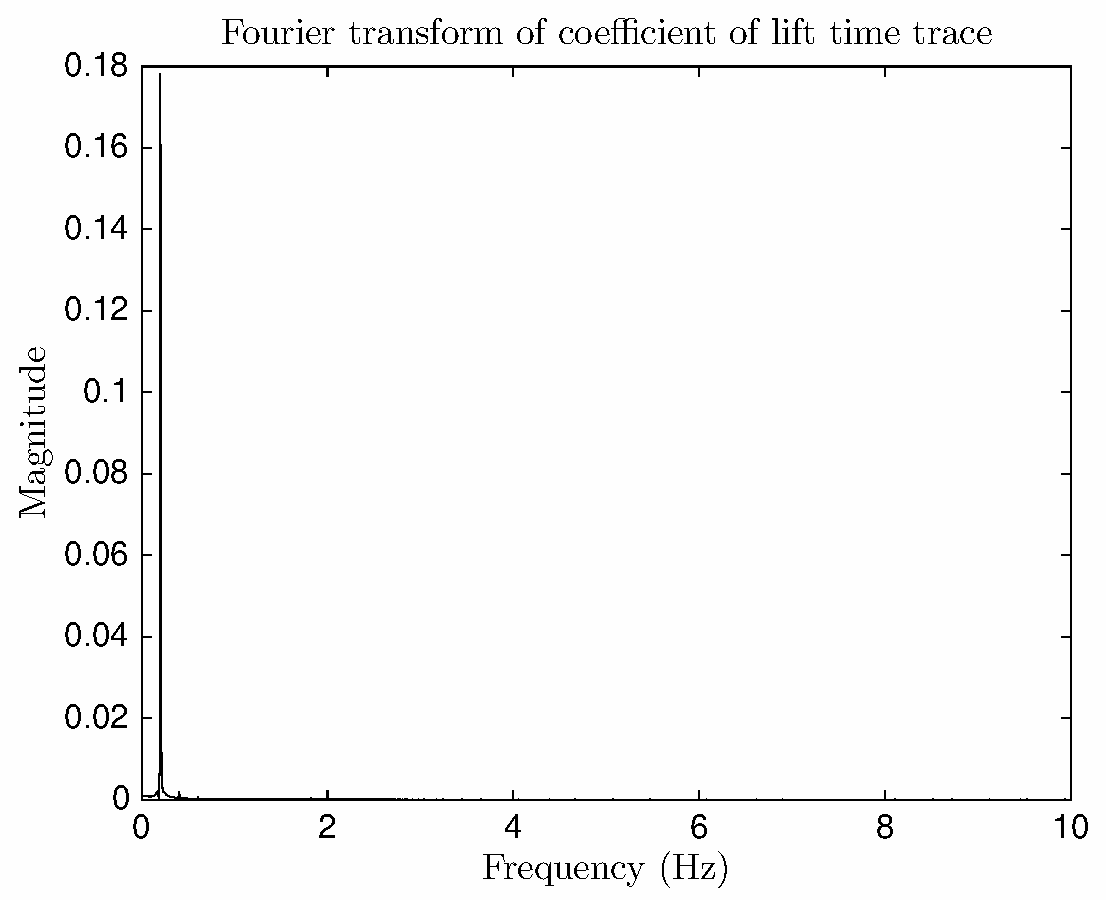
\includegraphics[scale=0.25]{FFT_100.eps}\\
%\caption{ Coefficient of lift time trace.}
  %\label{fig:SRe100.1}
  St = f = 0.202
\end{minipage}%
\begin{minipage}{.5\textwidth}
  \centering
  \fbox{\includemovie{5cm}{6cm}{SRe100.mp4}}
% \caption{figure}{Coefficient of drag time trace.}
  %\label{fig:SRe100.2}
\end{minipage}
\end{figure}
\end{frame}


%%%%%%%%%%%%%%%%%%%%%%%%%%%%%%%%


\section{Discussion}
\begin{frame}
\frametitle{Velocity profiles}
\underline{As Reynold's number increases:}
\pause
\begin{itemize}
\item Velocities at top and bottom of cylinder increases. 
\pause 
\item Seperation length increases. \\~\\
\end{itemize}
\pause
Beyond Reynold's number of 50, vortex shedding starts occuring.\\~\\
\pause

\end{frame}

\begin{frame}
\frametitle{Pressure profiles}
\underline{For Re=20, Re=50, Re=100:} \\
\pause
Relative pressure per unit density at leading edge was 0.74, 0.619, and 0.542 \si{\m^2\s^{-2}} respectively.\\~\\
\pause
The pressure difference on leading and trailing edge generates drag force. \\~\\
\pause
While, the pressure difference on top and bottom of the cylinder generates the lift force. \\~\\
\pause
Fluctuation in pressure occurred in Reynolds number beyond 50.
\end{frame}


\begin{frame}
\frametitle{Time traces and vortex shedding}
\begin{table}[H]
\centering
\resizebox{\textwidth}{!}{%
\begin{tabular}{|l|l|l|l|l|}
\hline
      & C\textsubscript{L}  & C\textsubscript{D}  &   frequency f/Hz & Strouhal Number St   \\ \hline
Re20  & 0.006          & 0.7815        & none & none \\ \hline
Re50  & 0.0136   & 0.5345        & 0.16    &  0.16    \\ \hline
Re100 & 0.136 $\leq  C\textsubscript{l} \leq$ -0.1048 & 0.493 & 0.202  & 0.202  \\ \hline
\end{tabular}
}
\caption{Shows the summary of results obtained.}
\label{mytable}
\end{table}
\pause
\underline{It can be established:}
\pause
\begin{itemize}
\item As Reynolds number increases C\textsubscript{D} decreases.
\item As Reynolds number increases C\textsubscript{L} increases.
\item Vortex shedding starts forming from Reynolds number 50.
\item As Reynold's number increases Strouhal number increases.
\end{itemize}


\end{frame}

%%%%%%%%%%%%%%%%%%%%%%%%%%%%%%%%%%%%%%%%%%%

\section{Final thoughts}


\begin{frame} 
\frametitle{Next Step?}
\pause
\underline{Further work to be done:}
\pause
\begin{itemize}
\item Explore Turbulence models. 
\item Set Variable boundary conditions.
\item Attempt to use a real bridge geometry.
\end{itemize}
\end{frame}

\begin{frame}
\frametitle{OpenFOAM vs ANSYS}
\begin{table}[]
\centering
\resizebox{\textwidth}{!}{%
\begin{tabular}{c|c|l|l|c|l|l}
                               & \multicolumn{3}{c|}{\textbf{OpenFOAM}}                    & \multicolumn{3}{c|}{\textbf{ANSYS}}                \\ \hline
\multirow{2}{*}{Advantages}    & \multicolumn{3}{c|}{1) Free license and open source}      & \multicolumn{3}{c|}{1) Good user interface}        \\
                               & \multicolumn{3}{c|}{2) Improves understanding of flow}    & \multicolumn{3}{c|}{2) More matured}               \\ \hline
\multirow{2}{*}{Disadvantages} & \multicolumn{3}{c|}{1) Lack of user interface}            & \multicolumn{3}{c|}{1) Expensive license}          \\
                               & \multicolumn{3}{c|}{2) No structured learning guidelines} & \multicolumn{3}{c|}{2) Can be used as a black box}
\end{tabular}%
}
\end{table}\end{frame}

\begin{frame}[allowframebreaks]
\frametitle{References}
\bibliographystyle{IEEEtran}
\bibliography{Reference.bib}
\end{frame}

\begin{frame}
Thank you for your undivided attention.
\end{frame}


\end{document}

%\begin{figure}
%\includemovie{10cm}{5cm}{p_Case1.mp4}
%\end{figure}
